\section{Introduction}
\label{sec:intro}
This report will discuss the notebook we made on restricted Hartree-Fock theory.
 We will walk trough the notebook step by step and discuss what we see there. 
 The same titles will be used, so you can follow along easily. 
 Relevant parts of the code will be displayed.

\section{Identifying the Molecule}
\label{sec:step1}
In this first step we initiated the class molecule, which will be equipped with 
the necessary methods to do all the calculations we will be required to do. 
A molecule object has several properties that need to be defined first. 


\begin{python}[caption={intitialising the molecule object},label={ls:Listing 1}]
    class molecule:
        def __init__(self, geom_file):
            if """pubchem""" in geom_file:
                self.id = psi4.geometry(geom_file)
            else:
                self.id = psi4.geometry(f"""
                {geom_file}
            
                units bohr
                """)
            self.id.update_geometry()
            self.wfn =  psi4.core.Wavefunction.build(self.id, 
                            psi4.core.get_global_option('basis'))
            self.basis = self.wfn.basisset()
            self.integrals = psi4.core.MintsHelper(self.basis)
            # only works for closed shell systems
            self.occupied = self.wfn.nalpha()  
            self.guessMatrix = "empty"
    
\end{python}
  

In Listing \ref{ls:Listing 1} we the \pythoninline{__innit__} method of the 
molecule class. It sets us up with some of the information we will need later, 
namely the \pythoninline{psi4.core.Molecule} representation as 
\pythoninline{self.id}. We also see the wave function, basis set, 
integrals, occupied orbitals and a guess matrix. 
Since we will be doing Hartree-Fock calculations, which involve a 
lot of iterations, the molecule object will need a way to store the Fock 
matrix from the last iteration. From there we can then start for the next 
iteration. Hence, the first method we actually have to define is a method that 
allows us to change this parameter.


\begin{python}[caption={setting the guessMatrix},label={ls:Listing 2}]
    def setGuess(self, new_guess):
        """
        sets the guessMatrix to a new value

        input:
        new_guess: numpy array that represents a new fock matrix
        """
        self.guessMatrix = new_guess
\end{python}

This is shown in Listing \ref{ls:Listing 2}. 

\section{Prerequisite Calculations}
\label{sec:step2}

In this section, we do some prerequisite calculations. These are relatively 
straightforward. In this step, we added some methods to the class that allow us to 
calculate important properties like the nuclear repulsion kinetic energy and so 
on. The commands used are directly implemented from the psi4 package. 
They are listed in Table \ref{tab:commands}

\begin{table}[hp]
    \centering
    \begin{tabular}{c|c}
        command & property \\
        \hline
        \pythoninline{self.id.nuclear_repulsion_energy()}| & nuclear repulsion energy \\
        \pythoninline{self.integrals.ao_overlap().np} & overlap matrix \\
        \pythoninline{self.integrals.ao_kinetic().np} & kinetic energy \\
        \pythoninline{self.integrals.ao_potential().np} & potential energy \\
        \pythoninline{self.displayE_kin() + self.displayE_pot()} & the core hamiltonian \\
        \pythoninline{self.integrals.ao_eri().np} & repulsion between electrons \\
    \end{tabular}
    \caption{Commands useed to calculate various properties}
    \label{tab:commands}
\end{table}
We will not list the code for the various methods here, however when they appear
 in later blocks of code we will mention them.

\section{The inital (Guess) Density Matrix}
\label{sec:step3}
We will skip ahead to the function that gives us the density matrix and start
 from there.

 
\begin{python}[caption={calculating the density matrix},label={ls:Listing 3}]
        class molecule(molecule):
            def getDensityMatrix(self):
                """
                generates the densitiy matrix on the AO level
                """
                C = self.getEigenStuff()[1]
                A = 2*np.einsum("pq, qr->pr", C[:, :self.occupied], 
                                C[:, :self.occupied].T, optimize=True)
                return A
\end{python}

This function uses the method \pythoninline{getEigenStuff}, which just calls 
the scipy function \pythoninline{linalg.eigh}. This solves the generalised 
eigenproblem posed by the Roothaan-Hall equations \eqref{eq:Roothaan-Hall}, 
for whatever matrix that is currently in the \pythoninline{self.guessMatrix} 
parameter.

\begin{equation}\label{eq:Roothaan-Hall}
    \boldsymbol{FC} = \boldsymbol{SC}\epsilon
\end{equation}

C in Listing \ref{ls:Listing 3} then refers to \textbf{C} in Equation 
\eqref{eq:Roothaan-Hall}. The first matrix for which we calculate the eigenvalues 
and eigenvectors is the core Hamiltonian, so this will have to be stored as the 
\pythoninline{self.guessMatrix} before proceeding. Now we are set to build a Fock 
matrix.

\section{Updating the Fock Matrix}
\label{sec:step4}


    
\begin{python}[caption={calculating the Fock matrix},label={ls:Listing 4}]
    class molecule(molecule):
        def displayFockMatrix(self):
            """Will display the Fock matrix"""
            coulomb = np.einsum("nopq,pq->no", 
                    self.displayElectronRepulsion(), 
                    self.getDensityMatrix(), optimize=True)
            exchange = np.einsum("npoq,pq->no", 
                    self.displayElectronRepulsion(), 
                    self.getDensityMatrix(), optimize=True)
            self.fockMatrix = self.displayHamiltonian() 
                            + coulomb - 0.5*exchange
            return self.fockMatrix
\end{python}
 
 
We see that the Fock-matrix uses some the density matrix and the electronic 
repulsion matrix and the Hamiltonian , which the molecule object calls with the 
methods seen in Section \ref{sec:step2}. Since the density matrix depends on the 
current \pythoninline{self.guessMatrix}, the Fock matrix will also depend on it. 
We can then see that the new Fock matrix is always derived from the previous one, 
given that we update it during each step of the iteration.
 
 \section{The SCF Energy}
 \label{sec:step5}
 From the Fock matrix we derived in the previous section, we can now calculate the electronic energy acoording to Equation \eqref{eq:energy}.
 
 \begin{equation} \label{eq:energy}
     E_{elek} = \frac{1}{2}\sum_{\mu\nu}D_{\mu\nu}*(H_{\mu\nu} + F_{\mu\nu})
 \end{equation}
 In python this looks like Listing \ref{ls:Listing 5}.
 
 
    
\begin{python}[caption={calculating the energy},label={ls:Listing 5}]
    class molecule(molecule):
        def getElectronicEnergy(self):
            """
            calculates the energy with the current fock matrix
            """
            sumMatrix = self.displayHamiltonian() 
                    + self.displayFockMatrix()
            return 0.5*np.einsum("pq,pq->", sumMatrix, 
                            self.getDensityMatrix())
\end{python}

The total energy is merely the sum of this electronic energy and the nuclear 
repulsion energy. We have a method for the latter defined in Section 
\ref{sec:step2}.
 
 \section{Test for Convergence}
 \label{sec:step6}
Now we only need to bring this all together to get the final energy. 
This is done in the function \pythoninline{iterator} as seen in Listing 
\ref{ls:Listing 6}.

 
   
\begin{python}[caption={iteration sequence},label={ls:Listing 6}]
    def iterator(target_molecule):
        """
        Function that performs the Hartree-Fock iterative calculations 
        for the given molecule.
        
        input:
        target_molecule: a molecule object from the class molecule
        """
        # setting up entry parameters for the while loop
        E_new = 0  
        E_old = 0
        d_old = target_molecule.getDensityMatrix()
        convergence = False
        E_list = []

        # step 2: start iterating
        itercount = 0
        while not convergence and itercount < 50:

            # calculating block: calculates energies
            E_new = target_molecule.getElectronicEnergy()
            E_total = target_molecule.getTotalEnergy()

            # generating block: generates new matrices
            F_n =  target_molecule.displayFockMatrix()
            target_molecule.setGuess(F_n)
            d_new = target_molecule.getDensityMatrix()

            # comparing block: "Are we there yet?"
            rms_D = np.einsum("pq->", np.sqrt((d_old - d_new)**2))
            if abs(E_old - E_new) < 1e-6 and rms_D < 1e-4:
                convergence = True


            # maintenance block: keeps everything going
            print(f"""iteration: {itercount}, E_tot: {E_total: .8f}, 
                        E_elek: {E_new: .8f}, 
                        deltaE: {E_new - E_old: .8f}, 
                        rmsD: {rms_D: .8f}""")
            E_old = E_new
            d_old = d_new
            E_list.append(E_new)
            itercount += 1
        
        return E_list
\end{python}

First we need to set up the parameters before we start iterating. That is done in 
the first block of code. Then we start a while loop, that will stop iterating once
we have reached convergence, or when we have reached the maximum amount of 
iterations. Inside the loop, we see four blocks of code. The calculating block 
provides us with the energy of the molecule for the given 
\pythoninline{self.guessMatrix}. The next block will generate new matrices for 
the next iterative step. In the comparing block we check the conditions for 
convergence. For this we need four values, the old and new energies and the old 
and new distance matrices. For more information, see Subsection 
\ref{subsec:step6.1}. For now we will continue to walk trough the code. 
After the comparing block we move to the final block, which sets us up for the 
next iteration. This iterations energy is stored, as well as the density matrix. 
We print out a line that summarises all the relevant values for this iteration. 
We can then move on to the next iterative step until the while loop finds one of 
its conditions is no longer met.
 
 \subsection{On Comparing Values}
 \label{subsec:step6.1}
 In Listing \ref{ls:Listing 6} we can see that there is a difference in the
 citeria for the density matrix and the energy. The reason here has to do with the way these 
 differences are calculated. We notice that the energy is calculated from the
 density 
 Indeed we see in Equation \ref{eq:energy} that the energy is calculated using a 
 product of the Fock matrix with the density matrix, when this Fock matrix is 
 already contains the density matrix as can be seen in Equation 
 \ref{eq: fock matrix}. 
 
 \begin{equation} \label{eq: fock matrix}
     F_{\mu\nu} = H_{\mu\nu} + \sum^{AO}_{\lambda\sigma}[(\mu\nu|\lambda\sigma) - \frac{1}{2}(\mu\lambda|\nu\sigma)]
 \end{equation}
criterion for the density matrix is the stricter criterion, even
 
 \section{Some examples}
 \label{sec: examples}
 In this section, we will display some of the results from our calculations for 
 two example systems, water and methane. We will give a display of the output as 
 generated by the functions we discussed above.
 
 \subsection{water}
 \label{subsec:water}

\begin{python}[caption={iterations for water},label={ls:Listing 7},basicstyle=\scriptsize]
0, E_tot: -73.28579642, E_elek: -81.28816348, deltaE: -81.2881634, rmsD:  14.05298222
1, E_tot: -74.82812538, E_elek: -82.83049244, deltaE: -1.54232896, rmsD:  3.17285816 
2, E_tot: -74.93548800, E_elek: -82.93785506, deltaE: -0.10736262, rmsD:  0.65858574 
3, E_tot: -74.94147774, E_elek: -82.94384480, deltaE: -0.00598974, rmsD:  0.24093051 
4, E_tot: -74.94197200, E_elek: -82.94433906, deltaE: -0.00049425, rmsD:  0.08612099
5, E_tot: -74.94205606, E_elek: -82.94442312, deltaE: -0.00008407, rmsD:  0.04061885
6, E_tot: -74.94207442, E_elek: -82.94444148, deltaE: -0.00001836, rmsD:  0.01827516
7, E_tot: -74.94207865, E_elek: -82.94444571, deltaE: -0.00000423, rmsD:  0.00892060
8, E_tot: -74.94207963, E_elek: -82.94444669, deltaE: -0.00000098, rmsD:  0.00425406
9, E_tot: -74.94207986, E_elek: -82.94444692, deltaE: -0.00000023, rmsD:  0.00205358
10, E_tot: -74.94207991, E_elek: -82.94444697, deltaE: -0.00000005, rmsD:  0.00098889
11, E_tot: -74.94207992, E_elek: -82.94444699, deltaE: -0.00000001, rmsD:  0.00047710
12, E_tot: -74.94207993, E_elek: -82.94444699, deltaE: -0.00000000, rmsD:  0.00023011
13, E_tot: -74.94207993, E_elek: -82.94444699, deltaE: -0.00000000, rmsD:  0.00011102
14, E_tot: -74.94207993, E_elek: -82.94444699, deltaE: -0.00000000, rmsD:  0.00005356
\end{python}
Here we see the the amount of iterations before the convergence is reached and 
all parameters calculated during that iteration. Furtermore we can use the 
\pythoninline{oeprop} method to get the dipole and nuclear charges. The dipole 
moment is given in e\AA, the charge is given in e, where e is the elemental 
charge.

\begin{table}[ht]
    \centering
    \begin{tabular}{c|c}
         total dipole moment & 0.6034  \\
         \hline
         nuclear charges &  \\ 
         \hline
         O & -0.25302 \\
         H & 0.12651 \\
         H & 0.12651 \\
    \end{tabular}
    \caption{Some properties of water}
    \label{tab:number2}
\end{table}

\begin{figure}
    \centering
    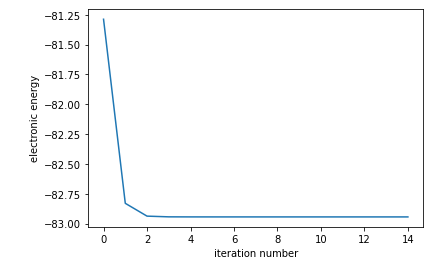
\includegraphics[width=0.5\textwidth]{content/Capture.PNG}
    \caption{convergence for water}
    \label{fig:convergence1}

\end{figure}
\subsection{methane}
\label{subsec:methane}
 
\begin{python}[caption={iterations for methane},label={ls:Listing 8},basicstyle=\scriptsize]
0, E_tot: -36.08344857, E_elek: -49.58075304, deltaE: -49.58075304, rmsD:  35.9980315
1, E_tot: -39.56451342, E_elek: -53.06181788, deltaE: -3.48106485, rmsD:  4.73662689
2, E_tot: -39.72183632, E_elek: -53.21914079, deltaE: -0.15732290, rmsD:  0.79654919
3, E_tot: -39.72669300, E_elek: -53.22399746, deltaE: -0.00485667, rmsD:  0.14041648
4, E_tot: -39.72684535, E_elek: -53.22414982, deltaE: -0.00015236, rmsD:  0.02394664
5, E_tot: -39.72685016, E_elek: -53.22415462, deltaE: -0.00000480, rmsD:  0.00443984
6, E_tot: -39.72685031, E_elek: -53.22415477, deltaE: -0.00000015, rmsD:  0.00072904
7, E_tot: -39.72685032, E_elek: -53.22415478, deltaE: -0.00000001, rmsD:  0.00014205
8, E_tot: -39.72685032, E_elek: -53.22415478, deltaE: -0.00000000, rmsD:  0.00002652
\end{python}
 
 \begin{table}[ht]
    \centering
    \begin{tabular}{c|c}
         total dipole moment & 0.0000  \\
         \hline
         nuclear charges &  \\ 
         \hline
         C & -0.26031 \\
         H & 0.06508 \\
         H & 0.06508 \\
         H & 0.06508\\
         H & 0.06508 \\
    \end{tabular}
    \caption{Some properties of methane}
    \label{tab:number2}
\end{table}

